%data manipulation towards the results, is this still methodology?

Post-acquisition, the \gls{csv} files were imported into Python using the pandas library. Column headers were standardized, and data integrity checks (duplicate removal, timestamp validation) were performed. However, the nature of the data is more complicated than that and required cleaning and manipulation for better understanding. 

To better illustrate this process, the next set of figures show examples for a single coordinate point (G6 from figure \ref{fig:fieldmapping_b}) which is representative of all the other coordinates data sets.

First, Figure \ref{fig:G6_BvsTime_raw} depicts the raw data in time for both runs, backwards on the left, forward on the right. A noticeable remark is the appearance of 2 outliers that are present along all data sets, suggesting cleaning to be workable. These outliers were removed with a quick exponential fit to use as baseline and remove residuals where the value was greater than $3\sigma$. Another remark was the fact that, excess measurements were taken at the beginning and end of each measuring run, most visible on the left side where a sudden plateau appears. This has to be cut as well, done by removing the leading/trailing near-constant flux checking with nearest neighbors withing a tolerance of 1 flux unit. 

%Figure \ref{fig:G6_BvsTime_raw}
%Assets/G6betterPlots/G6_BvsTime_raw.png
\begin{figure}[hbt!]
	\centering
	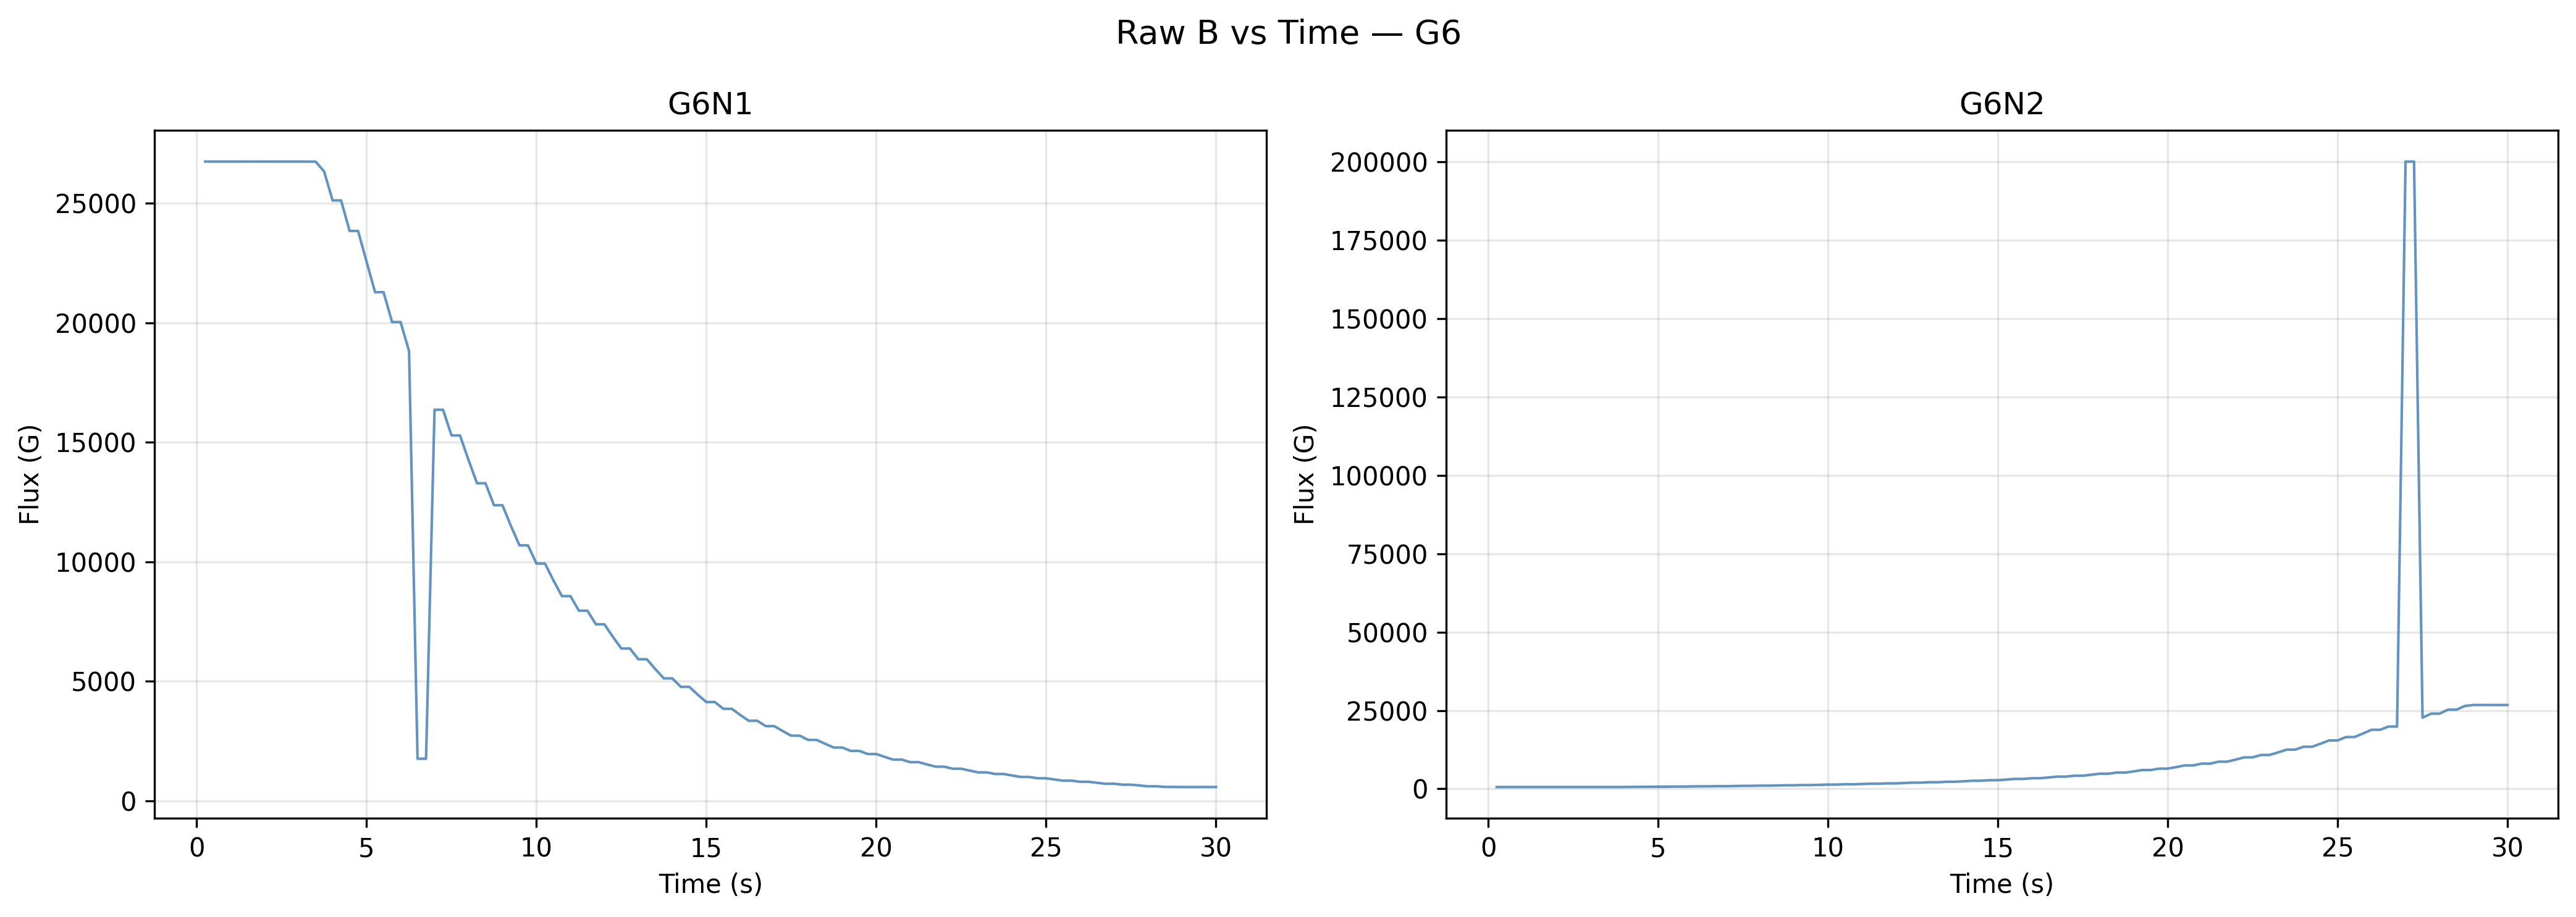
\includegraphics[width=0.95\textwidth]{Assets/G6betterPlots/G6_BvsTime_raw.png}
	\caption{Raw magnetic field measurements at coordinate G6 as a function of time. The left panel corresponds to the backward run and the right panel to the forward run. Two clear outliers are visible and appear consistently across all datasets.}
	\label{fig:G6_BvsTime_raw}
\end{figure}

Once both problems removed, the velocity of the patient couch with our fixture was calculated assuming constant speed by averaging the total time with the total distance (1252.0 mm) on each run. This allowed for conversion of the time axis to position along the couch, Figure \ref{fig:G6_BvsPosition} shows this plot. However, notice that some of the points on the plot are repeated making the plot look a bit step like, this in turn distorts the gradient calculations as central difference no longer works, as seen in Figure \ref{fig:G6_gradB}. This repetition arises from the resolution factor of our gaussmeter probe, set to 1 every 0.25s (4Hz) for such high field strength was to little resulting in saturation of the instrument. The repeated points mostly follow a pattern making pairs of data, a solution was implemented, separating the repeating points on 2 different runs, effectively making our measurement rate 1 every 0.50s (2Hz). 

%Figures \ref{fig:G6_BvsPosition} and Figure \ref{fig:G6_BvsPosition} 
%Assets/G6betterPlots/G6_BvsPosition.png
%Assets/G6betterPlots/G6_gradB.png


\begin{figure}[hbt!]
	\centering
	\subfloat[$B$ as a function of couch position.\label{fig:G6_BvsPosition}]{
		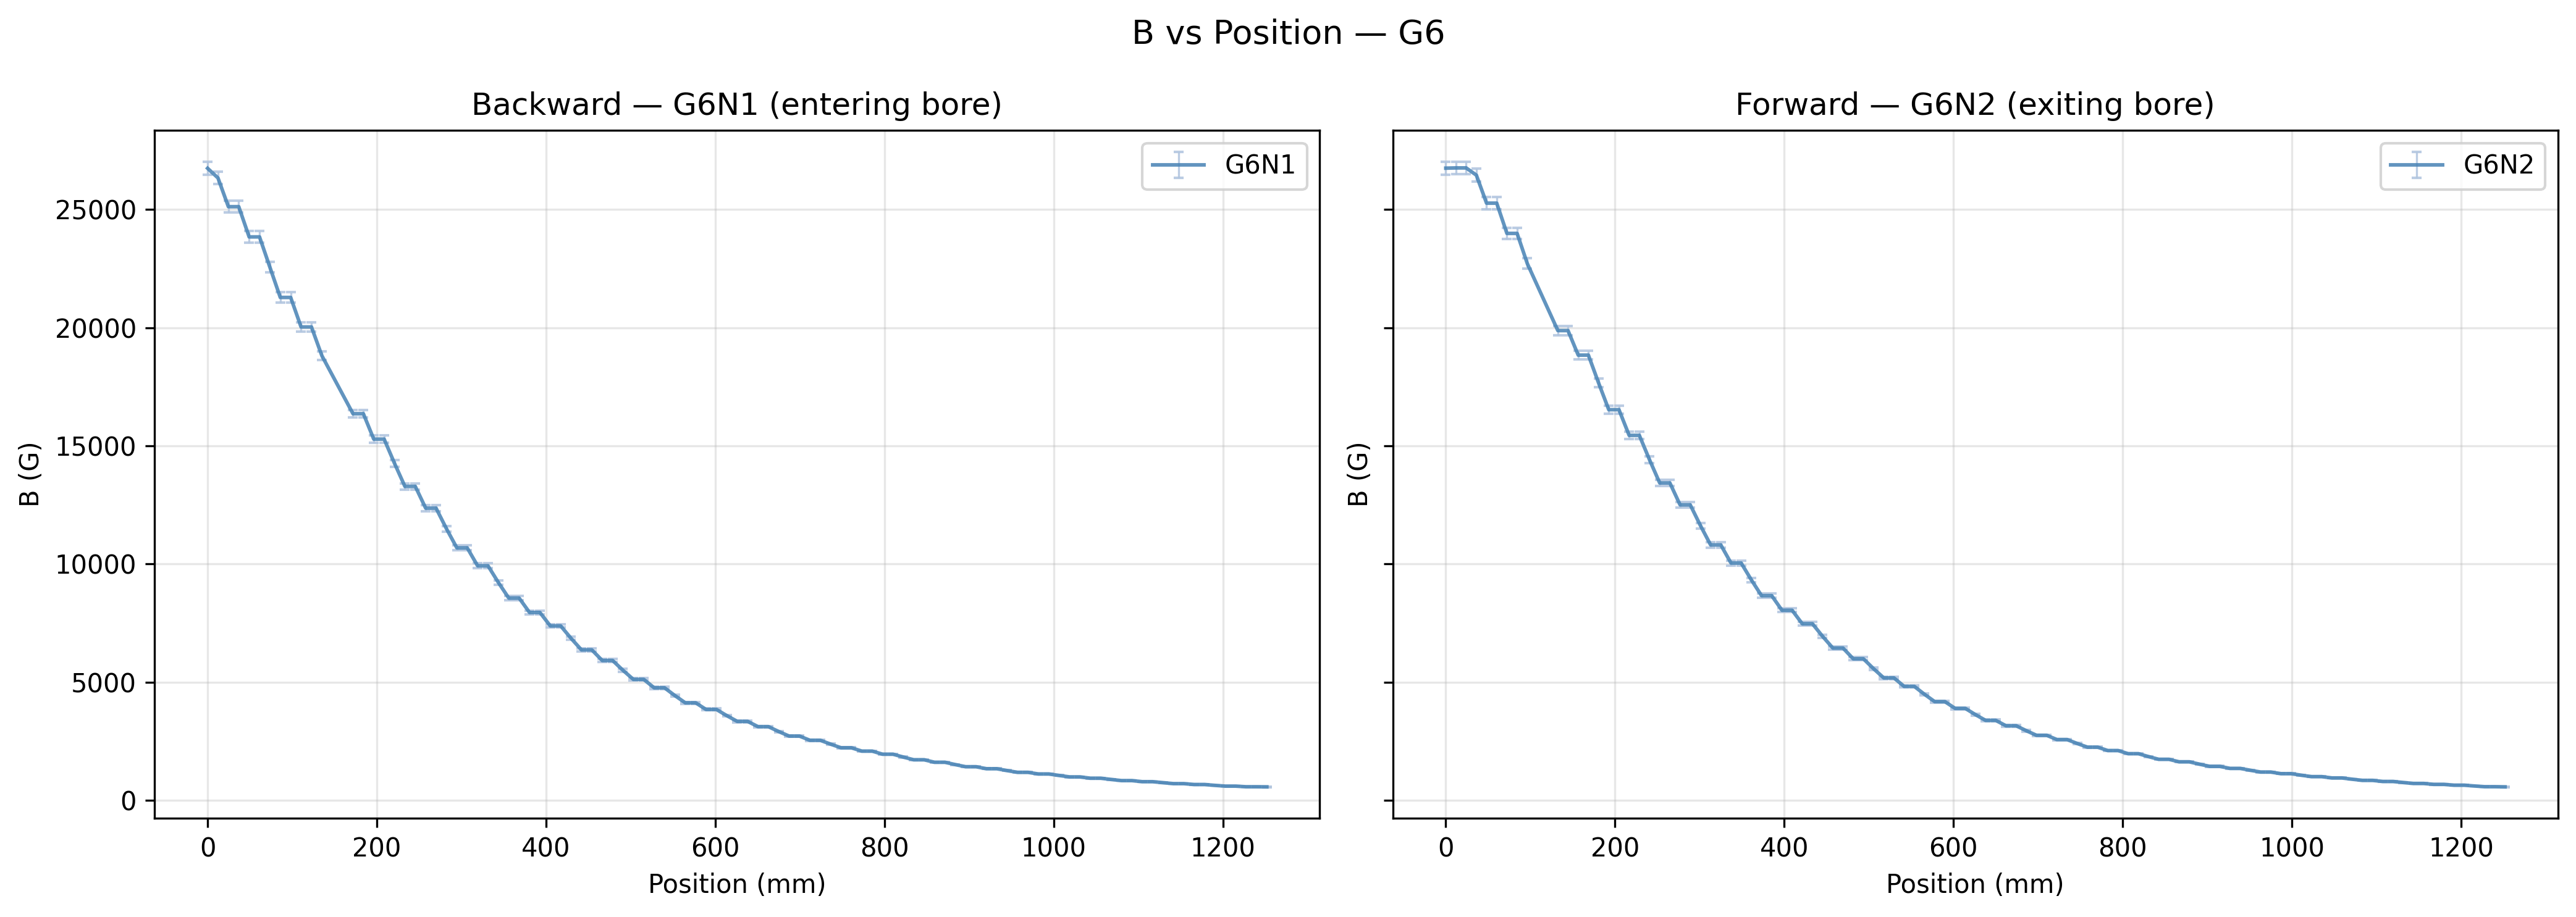
\includegraphics[width=0.95\textwidth]{Assets/G6betterPlots/G6_BvsPosition.png}
	}
	\hfill
	\subfloat[$\nabla B$ computed from the positional data.\label{fig:G6_gradB}]{
		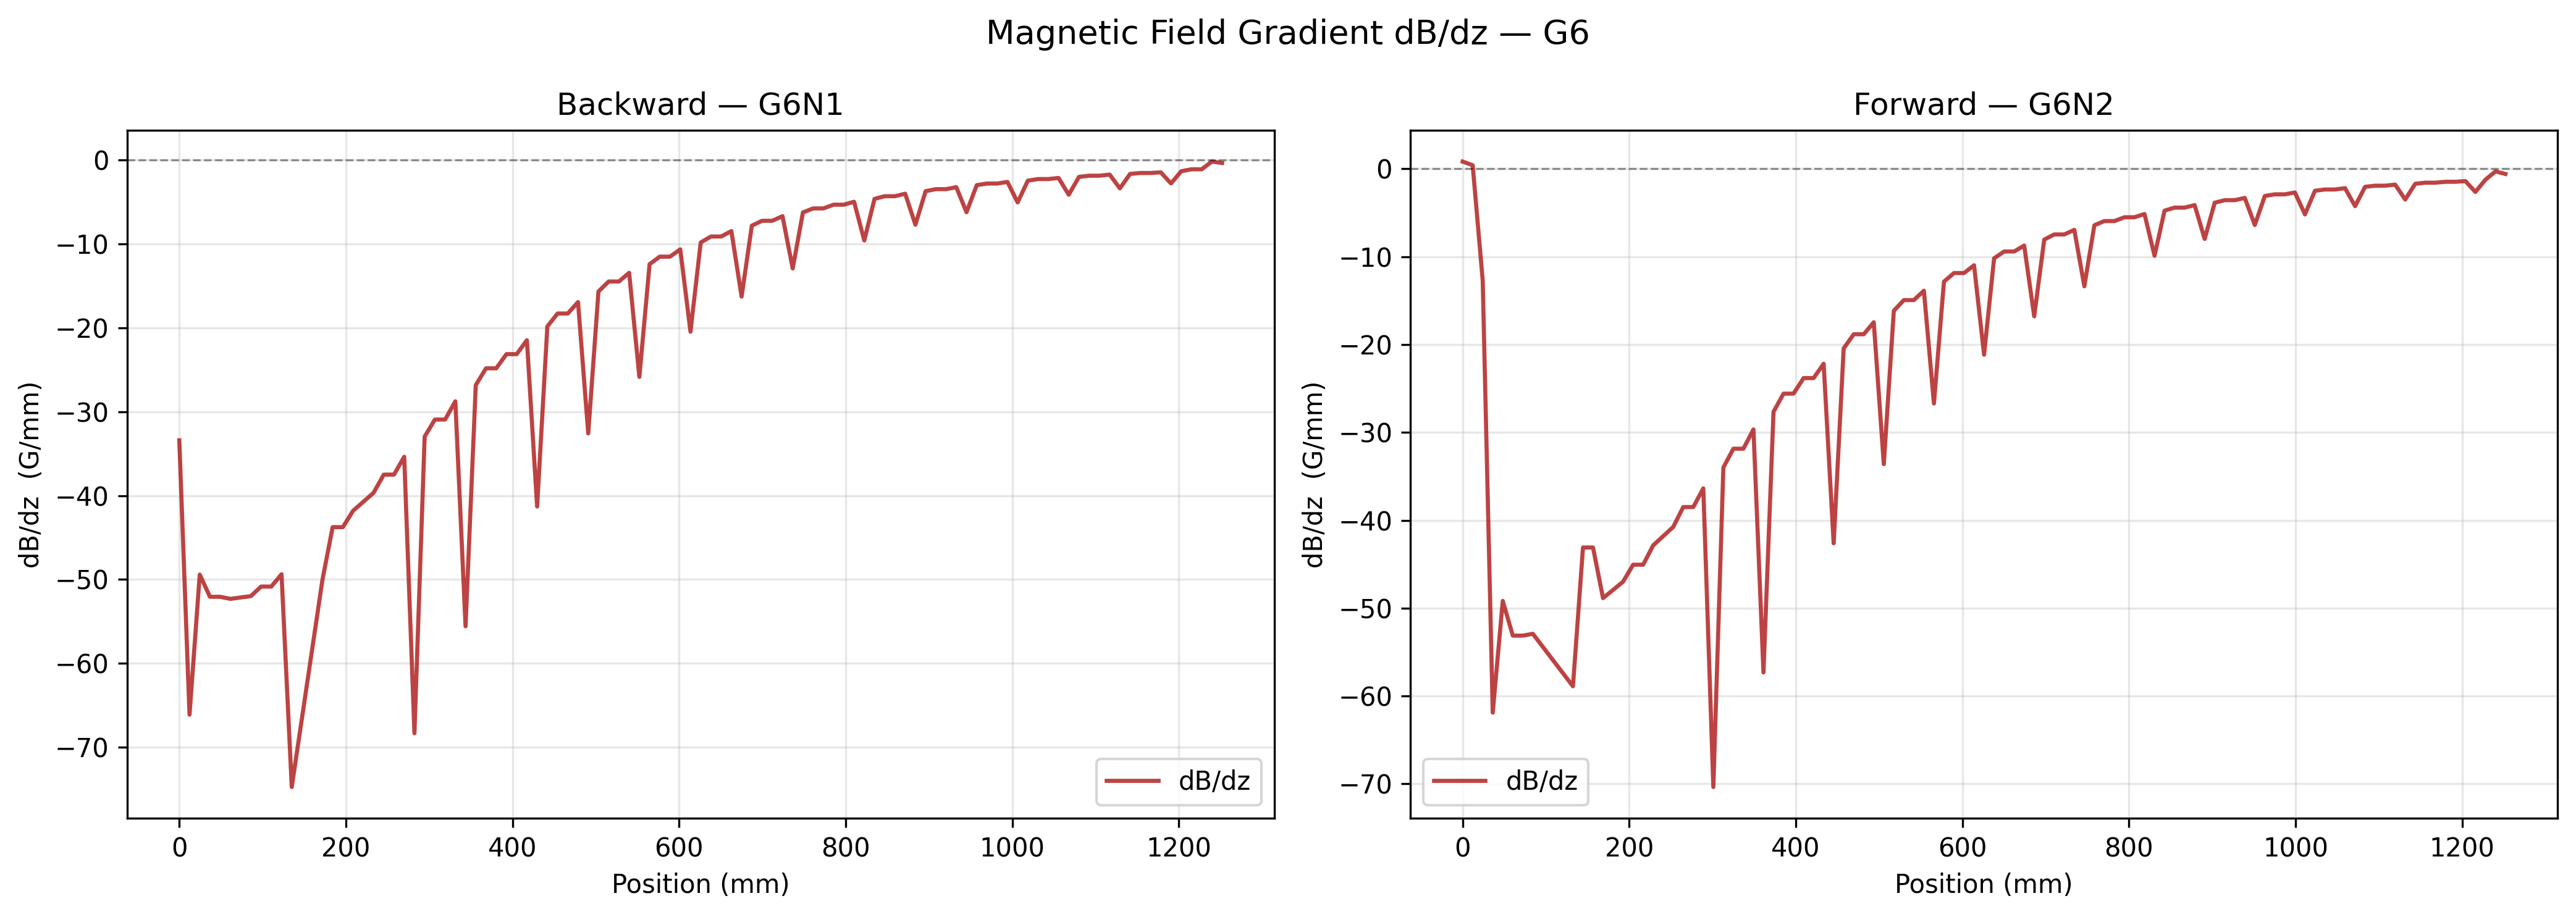
\includegraphics[width=0.95\textwidth]{Assets/G6betterPlots/G6_gradB.png}
	}
	
	\caption[Magnetic field and gradient before separation]{Magnetic field and corresponding gradient along the measurement path after converting time to position but prior to separating repeated measurements.}
	\label{fig:G6_position_pair}
\end{figure}

\FloatBarrier